\documentclass[aps,prx,reprint,superscriptaddress,longbibliography]{revtex4-2}

% ── Encoding & fonts ──
\usepackage[utf8]{inputenc}
\usepackage[T1]{fontenc}
\usepackage{microtype}

% ── Math ──
\usepackage{amsmath,amssymb,amsfonts}

% ── Tables ──
\usepackage{booktabs}
\usepackage{array}
\usepackage{multirow}
\usepackage{dcolumn}
\usepackage{makecell}

% ── Graphics ──
\usepackage{graphicx}
\graphicspath{{figures/}}

% ── Code listings ──
\usepackage{listings}
\lstset{
  basicstyle=\ttfamily\small,
  breaklines=true,
  frame=single,
  columns=fullflexible,
}

% ── Misc ──
\usepackage{xcolor}

% ── Custom commands ──
\newcommand{\Corr}{\mathrm{Corr}}
\newcommand{\SliceC}{\mathrm{SliceC}}
\newcommand{\TG}{\mathrm{TG}}
\newcommand{\sg}{\mathrm{sg}}

% ══════════════════════════════════════════════════════════════════════
\begin{document}

% ══════════════════════════════════════════════════════════════════════
% Front Matter (REVTeX 4.2 format)
% ══════════════════════════════════════════════════════════════════════

\title{ExactK: Iso-$K$ Hinge Loss for Robust $K$-Leakage Reduction\\in QEC Neural Decoders}

\author{Mohammad Albataineh}
\affiliation{Independent Researcher}
\email{albatainehm1@my.smccd.edu}

\date{\today}

\begin{abstract}
Neural decoders for quantum error correction on surface codes can exploit syndrome count~$K$---the number of triggered detectors---as a statistical shortcut, encoding density information into representations intended for spatial error topology. This \emph{K-leakage} confounds training diagnostics and may reduce the robustness benefits that motivate learned decoders over conventional matching-based methods. We report a systematic study of K-leakage mitigation in a bipartite factor-graph decoder trained on surface codes with correlated crosstalk noise. Across 28 development iterations, we evaluated 14 mitigation mechanisms spanning five families: global decorrelation, null-space alignment, K-orthogonalization, gradient shielding, and architectural factorization. None reliably reduced K-leakage while preserving topology across seeds at the required effect size---a consequence, our analysis indicates, of syndrome count being physically meaningful rather than purely spurious, so that interventions targeting global $Z$--$K$ dependence inevitably damage legitimate covariance.

We introduce ExactK, an auxiliary iso-$K$ hinge loss that mines training pairs exclusively from samples sharing identical syndrome count ($\Delta K = 0$). Because within-pair $K$ variation is removed by construction, ranking improvements under the auxiliary loss cannot be explained by pairwise $K$ differences. In the tested regime ($d{=}5$, $d{=}7$, $p{=}0.04$, correlated noise), ExactK reduces linear $K$-leakage by $31.2\%$ at $d{=}5$ (paired bootstrap 95\% CI: $[-46.3\%, 61.2\%]$, 10~seeds), $23.4\%$ at $d{=}7$ with the same hyperparameters (paired bootstrap 95\% CI: $[-51.4\%, 51.4\%]$, 10~seeds), and $45.0\%$ on unseen holdout seeds (paired bootstrap 95\% CI: $[-31.9\%, 60.7\%]$), with zero topology collapses across all validated ExactK experiments. The mechanism operates entirely in the forward pass, requiring no gradient surgery, no architectural modification, and no adversarial training.
\end{abstract}

\maketitle

% ══════════════════════════════════════════════════════════════════════
% Section 1: Introduction
% ══════════════════════════════════════════════════════════════════════

\section{Introduction}

\subsection{QEC Decoding and the Oracle Advantage}

Fault-tolerant quantum computing requires quantum error correction (QEC), in which redundantly encoded logical qubits are protected by repeated syndrome measurement and real-time decoding~\cite{PLACEHOLDER_qec_review}. The surface code~\cite{PLACEHOLDER_surface_code} is the leading candidate architecture for near-term implementations, owing to its high threshold under local noise and its planar layout compatible with superconducting qubit hardware.

The standard decoder for surface codes is minimum-weight perfect matching (MWPM)~\cite{PLACEHOLDER_mwpm}, which constructs a matching graph from the \emph{detector error model} (DEM)---a complete probabilistic description of which errors trigger which detectors and with what probability. MWPM's strength is precisely its \emph{oracle advantage}: it operates on exact knowledge of the noise structure. When the DEM is accurate, MWPM is efficient, well-understood, and provably optimal for independent Pauli noise on the matching graph~\cite{PLACEHOLDER_mwpm_optimality}.

Neural decoders offer a complementary approach. Rather than requiring an explicit DEM, a learned decoder can in principle extract decoding strategies directly from syndrome data~\cite{PLACEHOLDER_nn_decoder_survey}. This is appealing in settings where the noise model is uncertain, drifts over time, or contains correlations that MWPM approximates only through clique expansion of hyperedges~\cite{PLACEHOLDER_correlated_noise}. Recent work has demonstrated neural decoders based on multi-layer perceptrons~\cite{PLACEHOLDER_mlp_decoder}, graph neural networks~\cite{PLACEHOLDER_gnn_decoder}, recurrent architectures~\cite{PLACEHOLDER_rnn_decoder}, and transformers~\cite{PLACEHOLDER_transformer_decoder}, with several approaching MWPM accuracy on specific benchmarks.

However, the flexibility that allows neural decoders to learn from data also allows them to learn \emph{shortcuts}~\cite{PLACEHOLDER_shortcut_learning}. In particular, syndrome count~$K$---the total number of triggered detectors in a given measurement round---is a strong statistical predictor of the logical error probability $P(\text{error} \mid K)$. A decoder that simply learns this density lookup, without extracting any spatial structure from the syndrome pattern, can achieve deceptively good in-distribution accuracy while failing to generalize and offering no advantage over a trivial baseline.

\subsection{The $K$-Leakage Problem}
\label{sec:kleakage}

We define \emph{K-leakage} as the presence of syndrome-count information in the model's topology-intended internal representation. In our decoder architecture (Section~\ref{sec:background}), the model output is decomposed as
\begin{equation}
\hat{y} = f_{\text{prior}}(K) + \alpha \cdot z,
\end{equation}
where $f_{\text{prior}}(K)$ is a frozen density lookup and $z$ is the \emph{residual logit}---the normalized output of the topology channel after K-conditional standardization. The residual $z$ is intended to capture spatial error structure only. K-leakage occurs when $z$ still encodes~$K$, so that the model's supposed topology signal partly reduces to a density shortcut.

To measure K-leakage, we use a \emph{linear probe score}~$G_1$, defined as the five-fold cross-validated $R^2$ of a Ridge regression $z \to K$ evaluated on an independent held-out probe set of $N{=}4096$ samples. The probe input is the exact tensor used by the model for prediction---the normalized residual logit after removal of the density prior. $G_1 \in [0, 1]$, where $G_1{=}0$ indicates no linear $K$-information in~$z$. In the later selector-era analyses, values below $0.015$ define the ``organic clean'' regime in which the residual carries negligible linear $K$-dependence; earlier Day~55 stabilization used a stricter historical pass threshold of $0.01$ for probe qualification.

We emphasize that $G_1$ captures \emph{linear} leakage only. Earlier diagnostics using a nonlinear probe (a two-layer MLP trained to predict $K$ from~$z$) revealed that nonlinear $K$-predictability persists even when the linear component is fully removed. $G_1$ should therefore be understood as a \emph{conservative lower bound} on total K-leakage---it measures the dominant mode reliably and transparently, but does not capture higher-order dependence. The linear probe was adopted because it proved substantially more stable across epochs than the MLP probe, which exhibited order-of-magnitude fluctuations that rendered it unsuitable for epoch-level monitoring.

K-leakage is problematic for several reasons. It inflates apparent in-distribution performance, since $K$ is predictive of $Y$ independently of topology. It may degrade out-of-distribution robustness in settings where the $K$--$Y$ relationship shifts. And it obscures the degree to which the decoder has learned genuine spatial structure, making it difficult to assess whether a neural decoder offers any advantage over a density-only baseline.

\subsection{Prior Mitigation Attempts: A Systematic Falsification}
\label{sec:prior_attempts}

Over the course of this project, we evaluated 14~distinct mechanisms for reducing K-leakage, drawn from five methodological families. Each mechanism was tested on 3--10 random seeds with explicit topology safety checks (absence of topology collapse, defined as a significant degradation of within-$K$-slice predictive structure under $K$-matched scrambling). Table~\ref{tab:families} summarizes the families, their best outcomes, and their primary failure modes.

\begin{table*}
\caption{K-leakage mitigation families tested prior to ExactK. All 14 mechanisms failed to achieve reliable leakage reduction while preserving topology across seeds at the required effect size.}
\label{tab:families}
\renewcommand{\arraystretch}{1.3}
\centering
\begin{tabular*}{\textwidth}{@{\extracolsep{\fill}} l l l l @{}}
\hline\hline
Family & Mechanisms tested & Best outcome & Primary failure mode \\
\hline
Global reg./decorrelation & \makecell[l]{$\Corr(Z,K)^2$, GRL,\\hysteresis gating} & $+13.6\%$ $G_1$ reduction & \makecell[l]{Cannot separate physics\\from shortcut $K$-dep.} \\[4pt]
Null-space alignment & Null-space loss (4 variants) & Solved on 1/3 seeds & Seed-dependent topology loss \\[4pt]
K-orthogonalization & \makecell[l]{Rolling/EMA/frozen/\\epoch/ProbeSet $\beta$} & $-14\%$ to $-56\%$ (worse) & \makecell[l]{$\beta$ estimation too\\noisy or stale} \\[4pt]
Gradient shielding & \makecell[l]{Hard/soft/adaptive\\projection} & \makecell[l]{$+59.3\%$ (3 seeds);\\$-54.2\%$ (10 seeds)} & \makecell[l]{$K$-gradient carries topology\\on ${\sim}50\%$ of seeds} \\[4pt]
Arch.\ factorization & \makecell[l]{Split head +\\nuisance siphon} & $+29.9\%$ (1 collapse) & \makecell[l]{Siphon inert; regularizer\\was active ingredient} \\
\hline\hline
\end{tabular*}
\renewcommand{\arraystretch}{1.0}
\end{table*}

The central lesson from this falsification sequence is that syndrome count~$K$ is \emph{physically meaningful} in surface-code decoding: higher $K$ genuinely correlates with higher error probability because more syndrome triggers indicate more physical errors. Any intervention that penalizes the \emph{global} dependence between $z$ and $K$---whether through correlation penalties, adversarial training, gradient projection, or representation factorization---risks destroying legitimate covariance alongside the shortcut. Gradient shielding illustrated this most directly: projecting out the $K$-collinear component of the gradient improved leakage on seeds where the leakage was purely parasitic, but damaged topology on seeds where the $K$-collinear gradient carried genuine structural information.

K-orthogonalization ($\beta$ subtraction) failed for a different reason: estimating the linear regression coefficient $\beta$ between $z$ and $K$ from per-batch or per-epoch statistics proved fundamentally unreliable at the available sample sizes ($B{=}64$--$128$). The estimate was either too noisy (per-batch), too stale (frozen across epochs), or gated to inactivity by conservative safety thresholds.

These failures motivated a qualitatively different approach: rather than penalizing \emph{global} $Z$--$K$ dependence, restrict comparisons to samples with \emph{identical}~$K$, so that the auxiliary training signal carries no within-pair $K$ variation by construction.

\subsection{Contributions}

This paper makes the following contributions:

\begin{enumerate}
\item \textbf{ExactK iso-$K$ hinge loss.} We introduce an auxiliary forward-pass loss that mines training pairs exclusively from samples sharing identical syndrome count ($\Delta K{=}0$) and applies a hinge-margin ranking objective within these pairs. Because within-pair $K$ variation is removed by construction, ranking improvements under the iso-$K$ loss cannot be explained by pairwise $K$ differences. The mechanism requires no gradient surgery, no architectural modification, and no adversarial training---only a pair-mining step within each batch (Section~\ref{sec:method}).

\item \textbf{Systematic negative results.} We document the failure modes of 14 prior mechanisms across 5~families, providing a structured account of why global decorrelation, orthogonalization, and gradient shielding are unreliable for K-leakage reduction in QEC decoders. The root-cause analysis---that $K$ carries physically meaningful information that these methods cannot separate from shortcut dependence---motivates the local, within-$K$ design of ExactK (Section~\ref{sec:prior_mitigation}, Appendix~\ref{app:negative}).

\item \textbf{Multi-scale validation within the tested regime.} We validate ExactK at code distance $d{=}5$ (10~seeds, $+31.2\%$ median $G_1$ reduction), at $d{=}7$ using identical hyperparameters (10~seeds, $+23.4\%$), and on 10 unseen holdout seeds at $d{=}7$ ($+45.0\%$), with zero topology collapses across the 30-seed Day~69/70/75 validation suite and 960/960 alignment checks passing. All experiments use surface codes with correlated crosstalk noise at $p{=}0.04$ (Section~\ref{sec:experiments}).

\item \textbf{Checkpoint selection methodology.} We identify the \emph{Asymmetric Selection Paradox}---a pitfall in which multi-objective checkpoint selectors with heterogeneous pool criteria produce misleading inter-arm comparisons---and present a topology-aware selector that decouples leakage-reduction assessment from deployment checkpoint choice (Section~\ref{sec:selector}).
\end{enumerate}

% ══════════════════════════════════════════════════════════════════════
% Section 2: Background and Problem Formulation
% ══════════════════════════════════════════════════════════════════════

\section{Background and Problem Formulation}
\label{sec:background}

\subsection{Surface Codes and Decoding}

We consider the standard memory experiment on the rotated surface code~\cite{PLACEHOLDER_surface_code} at code distances $d \in \{5, 7\}$, with $r = d$ rounds of syndrome extraction. A distance-$d$ rotated surface code has $n_d = d^2$ data qubits, $d^2 - 1$ stabilizer measurements per round, and yields $n_{\mathrm{det}}$ detector events ($n_{\mathrm{det}} = 120$ at $d{=}5$, $n_{\mathrm{det}} = 336$ at $d{=}7$) and a single logical observable flip $Y \in \{0, 1\}$.

Circuits are generated using Stim~\cite{PLACEHOLDER_stim}, which produces a detector error model (DEM)---a list of independent error mechanisms, each annotating which detectors it triggers with what probability and whether it flips the logical observable. The DEM is the sufficient statistic for maximum-likelihood decoding and is used directly by MWPM~\cite{PLACEHOLDER_pymatching} via construction of a matching graph.

\paragraph{Notation.} Throughout, $d$~denotes code distance, $p$~the physical error rate, $K = \sum_{i=1}^{n_{\mathrm{det}}} x_i$~the syndrome count (total triggered detectors), $Y \in \{0,1\}$~the logical error label, and $\mathbf{x} \in \{0,1\}^{n_{\mathrm{det}}}$~the raw syndrome vector.

\subsection{Noise Model}

All experiments use the \emph{correlated crosstalk} noise model, which combines SD6-like independent depolarizing noise with correlated two-qubit errors:
\begin{equation}
p_{\text{ind}} = (1 - c) \cdot p, \qquad p_{\text{corr}} = c \cdot p,
\end{equation}
where $c = 0.5$ is the correlation strength. Independent noise follows the SD6 channel structure ($p_{1q} = 0.1\,p_{\text{ind}}$, $p_{2q} = p_{\text{ind}}$, $p_{\text{meas}} = p_{\text{ind}}$), while correlated noise is injected as $\texttt{CORRELATED\_ERROR}(p_{\text{corr}})\; X_{q_0} X_{q_1}$ after each two-qubit gate. The correlated component creates $k{>}2$ hyperedges in the DEM that MWPM must approximate via clique expansion~\cite{PLACEHOLDER_correlated_decoding}. All experiments use $p = 0.04$ and basis~$X$.

\subsection{Factor-Graph Neural Decoder}

We use a bipartite factor-graph decoder that represents the DEM directly as a bipartite graph with two node types:
\begin{itemize}
\item \textbf{Detector nodes}~$V_D$: one per detector event (including a virtual boundary node), with input feature $x_i \in \{0,1\}$ (syndrome bit).
\item \textbf{Error nodes}~$V_E$: one per merged error mechanism, with input feature $w_e$ (DEM matching weight $w = \ln((1-p_e)/p_e)$).
\end{itemize}

Each DEM error term becomes an error node connected to all detectors in its support set. Mechanisms with identical detector support and observable mask are merged via $p_{\text{merge}} = 1 - \prod_i (1 - p_i)$. This representation preserves $k{>}2$ hyperedge structure exactly, avoiding the information loss of clique expansion used by standard graph-based decoders.

\paragraph{Message passing.} The decoder applies $L{=}3$ bipartite message-passing layers. Each layer performs two aggregation steps:
\begin{widetext}
\begin{align}
\mathbf{h}_{E}^{(\ell+1)} &= \mathrm{LN}\!\left(\mathbf{h}_{E}^{(\ell)} + \mathrm{drop}\!\left(\mathrm{ReLU}\!\left(W_e \mathbf{h}_{E}^{(\ell)} + \mathrm{AGG}_{D \to E}\!\left(\sigma(\mathbf{w}_e) \odot \left(W_{D \to E}\,\mathbf{h}_{D}^{(\ell)}\right)\right) + \mathbf{b}_e\right)\right)\right), \\
\mathbf{h}_{D}^{(\ell+1)} &= \mathrm{LN}\!\left(\mathbf{h}_{D}^{(\ell)} + \mathrm{drop}\!\left(\mathrm{ReLU}\!\left(W_d \mathbf{h}_{D}^{(\ell)} + W_{E \to D}\,\mathrm{AGG}_{E \to D}\!\left(\mathbf{h}_{E}^{(\ell+1)}\right) + \mathbf{b}_d\right)\right)\right),
\end{align}
\end{widetext}
where $\mathrm{AGG}_{D \to E}$ is a weighted scatter-mean (D$\to$E messages scaled by $\sigma(w_e)$, the sigmoid of the DEM matching weight of the destination error node) and $\mathrm{AGG}_{E \to D}$ is an unweighted scatter-mean. The hidden dimension is $H{=}48$ and dropout is~$0.1$.

\paragraph{Readout.} Error nodes with $\texttt{observable\_mask} = \mathrm{True}$ (those whose error mechanism flips the logical observable) are selected for pooling. The readout is $\mathrm{concat}(\mathrm{mean}(\mathbf{h}_{E}^{\mathrm{obs}}), \mathrm{max}(\mathbf{h}_{E}^{\mathrm{obs}}))$, passed through a two-layer MLP with ReLU and dropout to produce a scalar logit.

\paragraph{Anti-leakage design.} The observable mask is used \emph{only} for readout pooling and is \emph{never} included as a message-passing feature. This prevents the model from learning a trivial shortcut through the mask.

\subsection{Density-Residual Decomposition}

The decoder's scalar logit is decomposed as
\begin{equation}
\hat{y} = f_{\text{prior}}(K) + \alpha \cdot z,
\end{equation}
where $f_{\text{prior}}(K)$ is a frozen per-bin lookup table estimating $\log(P(Y{=}1 \mid K) / P(Y{=}0 \mid K))$ from training data, $z$~is the \emph{residual logit} after K-Conditional Standardization (KCS), and $\alpha$~is a learned interpolation weight (a global scalar in the default configuration; optionally $K$-bin-conditioned via a learned lookup table). KCS normalizes the raw residual within each $K$-bin:
\begin{equation}
z_i = \frac{r_i - \mu_{K}[\mathrm{bin}(K_i)]}{\max\!\left(\sigma_{K}[\mathrm{bin}(K_i)],\; \sigma_{\text{floor}}\right)},
\end{equation}
where $\mu_K$ and $\sigma_K$ are per-bin batch statistics and $\sigma_{\text{floor}} = 0.1$. The residual~$z$ is the \emph{topology channel}: it is intended to encode spatial error structure that the density prior cannot capture. K-leakage occurs when $z$ still carries $K$-information despite the KCS normalization.

\subsection{Measuring $K$-Leakage: The $G_1$ Probe}

We measure linear K-leakage using a probe score $G_1$ defined as the five-fold cross-validated $R^2$ of a Ridge regression from $z$ to $K$, evaluated on an independent probe set of $N{=}4096$ samples generated with a deterministic seed:
\begin{equation}
G_1 = R^2_{\mathrm{cv}}\!\left(\mathrm{Ridge}(z \to K)\right).
\end{equation}
The probe input is the exact tensor~$z$ (the normalized residual logit after density-prior removal and KCS) that the model uses for prediction; in code this probe tensor is exposed as \texttt{logit\_residual\_norm}. $G_1 = 0$ indicates no linear $K$-information in~$z$. In the selector-era analyses, values below $0.015$ define the \emph{organic clean} regime, while the earlier Day~55 stabilization used a stricter historical pass threshold of $0.01$. The primary evaluation metric is the \emph{epoch-median~$G_1$}: for each seed, we take the median $G_1$ across all active-phase epochs ($\geq 6$), then report the median across seeds.

$G_1$ captures linear leakage only and should be understood as a conservative lower bound on total K-leakage (see Section~\ref{sec:kleakage}).

\subsection{TopologyGain}

TopologyGain (TG) measures whether the model exploits spatial structure beyond what syndrome count alone provides:
\begin{equation}
\TG = \overline{\SliceC}_{\text{clean}} - \overline{\SliceC}_{\text{scrambled}},
\end{equation}
where $\overline{\SliceC}$ is the mean within-$K$-slice C-statistic (concordance index, equivalent to AUROC computed separately within each syndrome-count bin) and \emph{scrambling} denotes $K$-matched permutation of detector-bit positions, which destroys spatial structure while preserving~$K$. A topology \emph{collapse} is detected when the difference in mean drop between the control arm and the treatment arm exceeds $0.10$. Note that \emph{topology collapse} is a scientific diagnostic concept; the selector pool label \texttt{TOPO\_FAIL} (Section~\ref{sec:selector}) is a distinct operational category denoting that no epoch survived the topology-floor filter, and does not necessarily indicate topology collapse in the diagnostic sense.

% ══════════════════════════════════════════════════════════════════════
% Section 3: Method — ExactK Iso-K Hinge Loss
% ══════════════════════════════════════════════════════════════════════

\section{Method: ExactK Iso-$K$ Hinge Loss}
\label{sec:method}

\subsection{Motivation: Why Global Decorrelation Fails}
\label{sec:prior_mitigation}

A natural approach to reducing K-leakage is to penalize the global dependence between $z$ and $K$---for example, by adding $\lambda \cdot \Corr(z, K)^2$ to the training loss. Our experiments with this and related global methods (Sec.~\ref{sec:prior_attempts}, Table~\ref{tab:families}) revealed a fundamental obstacle: syndrome count~$K$ is \emph{physically meaningful} in QEC\@. Higher $K$ genuinely indicates more errors, so $z$ and $K$ share legitimate covariance that carries topology-relevant information. A global penalty cannot distinguish this physics-linked covariance from shortcut dependence, and applying it aggressively enough to reduce $G_1$ consistently damages the topology signal.

This motivates a different strategy: rather than penalizing the global $z$--$K$ relationship, restrict all comparisons to samples with identical~$K$, so that the auxiliary training signal carries no within-pair $K$ variation by construction.

\subsection{Algorithm}

ExactK is an auxiliary hinge-margin ranking loss that operates on pairs of samples with identical syndrome count and opposite labels. Given a training batch with residual logits $z \in \mathbb{R}^B$, syndrome counts $K \in \mathbb{Z}^B$, and labels $Y \in \{0,1\}^B$:

\begin{enumerate}
\item \textbf{Partition} the batch into positive ($\mathcal{P} = \{i : Y_i = 1\}$) and negative ($\mathcal{N} = \{j : Y_j = 0\}$) index sets.
\item \textbf{Mine exact-$K$ pairs}: $\mathcal{S} = \{(i,j) : i \in \mathcal{P},\; j \in \mathcal{N},\; K_i = K_j\}$.
\item \textbf{Subsample} if $|\mathcal{S}| > M$: draw $M$ pairs uniformly at random.
\item \textbf{Compute hinge loss}:
\begin{equation}
\mathcal{L}_{\text{iso}} = \frac{\lambda_{\text{eff}}}{|\mathcal{S}'|} \sum_{(i,j) \in \mathcal{S}'} \max\!\bigl(0,\; m - (z_i - z_j)\bigr),
\end{equation}
where $\mathcal{S}'$ denotes the (sub)sampled pairs, $m$~is the hinge margin, and $\lambda_{\text{eff}}$ follows a schedule:
\begin{widetext}
\begin{equation}
\lambda_{\text{eff}} = \begin{cases} 0 & \text{if epoch} \leq 5 \;\text{(warmup)} \\ \lambda & \text{if } 5 < \text{epoch} \leq 8 \\ \lambda \cdot 0.85^{(\text{epoch} - 8)} & \text{if epoch} > 8 \end{cases}
\end{equation}
\end{widetext}
\end{enumerate}

The total training loss is $\mathcal{L} = \mathcal{L}_{\text{focal}} + \mathcal{L}_{\text{iso}}$, where $\mathcal{L}_{\text{focal}}$ is the focal loss~\cite{PLACEHOLDER_focal_loss} ($\gamma{=}2$) on the full batch.

\paragraph{Structural property.} Because every pair $(i,j) \in \mathcal{S}$ satisfies $K_i = K_j$, there is no within-pair $K$ variation. Ranking improvements under $\mathcal{L}_{\text{iso}}$ therefore cannot be explained by pairwise $K$ differences---only by features orthogonal to $K$ within each bin. This property holds by construction and does not depend on model architecture or training dynamics. We note, however, that the main loss $\mathcal{L}_{\text{focal}}$ still operates on all samples and can learn $K$-dependent features; ExactK constrains only the auxiliary ranking channel.

\subsection{Why $\Delta K = 0$ Is Essential}

We tested a relaxed variant, NearK ($|\Delta K| \leq 1$), which allows pairing between adjacent $K$ bins and yields approximately $2.6{\times}$ more pairs per batch (${\sim}123$ vs ${\sim}47$ at $d{=}5$, $B{=}64$). Despite the higher pair density, NearK performed dramatically worse than control in aggregate ($-155\%$ median~$G_1$) and caused topology collapse on seed~53000 (Section~\ref{sec:ablation_dk}). The reason is that adjacent $K$ bins have systematically different error probabilities, so $\Delta K{=}1$ pairs reintroduce the density confound: the model can satisfy the hinge margin by learning to predict ``higher $K$ implies higher error risk'' rather than learning spatial topology.

This ablation is the paper's central falsification result. It demonstrates that the strict $\Delta K{=}0$ constraint is not merely conservative---it is necessary for the mechanism's reliability.

\subsection{Pair Density}

A potential concern with exact-$K$ matching is pair sparsity. At extreme $K$ values (very low or very high syndrome count), few samples share the same~$K$, yielding zero pairs in those bins. In the Day~67 hard-seed ablation at $d{=}5$ with batch size $B{=}64$, ExactK produced ${\sim}47$ pairs per batch on average, versus ${\sim}123$ for NearK, with 100\% batch coverage (every batch contained at least one valid pair). The ranking signal is therefore concentrated in the mid-$K$ regime where most samples cluster, and this proved sufficient for reliable $G_1$ reduction. At $d{=}7$, the pair budget was increased to $M{=}512$ to compensate for the larger training setup.

\subsection{Production Hyperparameters}

\begin{table}[htbp]
\caption{ExactK production configuration.}
\label{tab:hyperparams}
\begin{ruledtabular}
\begin{tabular}{lll}
Parameter & Value & Notes \\
\hline
$\Delta K$ & 0 & Exact $K$ matching \\
$\lambda$ & 0.10 & Iso-$K$ loss weight \\
$m$ & 0.30 & Hinge margin (see Section~\ref{sec:ablation_margin}) \\
Decay & $0.85^{(\text{ep}-8)}$ for ep $> 8$ & Late-epoch pressure reduction \\
$M$ & 256 ($d{=}5$) / 512 ($d{=}7$) & Max pairs per batch \\
Warmup & 5 epochs & $\lambda_{\text{eff}}{=}0$ during base learning \\
Batch std. & Off (raw $z$) & See below \\
Epochs & 12 & 5 warmup + 7 active \\
\end{tabular}
\end{ruledtabular}
\end{table}

\paragraph{On batch standardization.} An alternative formulation standardizes $z$ before computing the hinge: $z' = (z - \bar{z}) / \sg(\hat{\sigma}_z)$, where $\sg$ denotes stop-gradient on the scale. This was tested as the SafeStd arm in Day~68. Standardization reduced aggregate improvement from $+26.6\%$ (raw~$z$) to approximately $0\%$, indicating that the magnitude of~$z$---not just its rank ordering---carries informative structure for the iso-$K$ objective. The production configuration therefore operates on raw~$z$.

\subsection{Scope and Non-Claims}

ExactK does not guarantee zero K-leakage. It reduces $G_1$ by $31$--$45\%$ on median in the tested regimes, with a minority of seeds showing increased leakage (Section~\ref{sec:adversarial}). It does not modify the model architecture, does not perform gradient surgery, and does not prevent the main loss from learning $K$-dependent features. The $G_1$ metric captures linear leakage; nonlinear leakage remains unmeasured by the current probe and is not directly targeted by ExactK.

% ══════════════════════════════════════════════════════════════════════
% Section 4: Experiments and Results
% ══════════════════════════════════════════════════════════════════════

\section{Experiments and Results}
\label{sec:experiments}

\subsection{Setup}

\paragraph{Data.} Surface code circuits at $d \in \{5, 7\}$, $p = 0.04$, $X$~basis, correlated crosstalk noise ($c{=}0.5$), generated via Stim~\cite{PLACEHOLDER_stim}. Training samples: $N_{\text{train}}{=}2048$ for $d{=}5$ experiments, $N_{\text{train}}{=}4096$ for $d{=}7$. An independent probe set of $N_{\text{probe}}{=}4096$ samples (deterministic seed) was used for all $G_1$ evaluations.

\paragraph{Arms.} Days~69 and 70 use three arms $\times$ 10~seeds: (A)~Control (no iso-$K$ loss, $\lambda{=}0$), (B)~ExactK with production hyperparameters, and (C)~a variant arm specified per experiment. Day~75 (holdout) uses two arms $\times$ 10~seeds: Control and ExactK only. The Day~67 $\Delta K$ ablation (Section~\ref{sec:ablation_dk}) is a separate Phase-1 falsification study on 4~hard seeds.

\paragraph{Seeds.} $d{=}5$ and $d{=}7$ experiments used seeds $\{47000, 49000, 49200, 50000, 51000, 52000, 53000, 54000, 55000, 56000\}$. The holdout experiment used seeds $\{60000, \ldots, 60009\}$, which were never used during development.

\paragraph{Hardware.} The $d{=}5$ canonical results were produced on CPU (Intel i7-14700HX, Windows~11). The $d{=}7$ canonical results were produced on GPU (NVIDIA RTX PRO 6000, 96\,GB VRAM, RunPod Ubuntu~24.04). Cross-platform reproduction may yield numerically different but qualitatively consistent results due to floating-point non-determinism (Appendix~\ref{app:repro}).

\paragraph{Evaluation.} The primary metric is the epoch-median~$G_1$: for each seed, the median of $G_1$ across active-phase epochs ($\geq 6$), then the median across seeds. The improvement $\Delta$ is computed as $(G_{1,\text{ctrl}} - G_{1,\text{prod}}) / G_{1,\text{ctrl}}$, where positive values indicate reduced leakage. We report paired bootstrap 95\% CIs for the median relative improvement using percentile intervals over seed-level paired resamples (100,000 resamples, random seed~42). For Day~69 and Day~70 experiment artifacts, the historical field name \texttt{G1\_raw\_probe} was mapped to the canonical \texttt{G1\_aligned} metric via the repository's \texttt{\_normalize\_epoch} compatibility function; Day~75 used \texttt{G1\_aligned} natively.

\subsection{Experiment 1: $d{=}5$ Primary Validation}

\begin{table}[htbp]
\caption{Aggregate results at $d{=}5$ (10~seeds, $N_{\text{train}}{=}2048$, epochs $\geq 6$).}
\label{tab:d5}
\begin{ruledtabular}
\begin{tabular}{llll}
Arm & Median $G_1$ & $\Delta$ vs Control & Topo.\ collapses \\
\hline
Control & 0.0154 & --- & 0/10 \\
\textbf{ExactK} & \textbf{0.0106} & \textbf{+31.2\%} & \textbf{0/10} \\
ExactK Gated & 0.0117 & +24.0\% & 0/10 \\
\end{tabular}
\end{ruledtabular}
\end{table}

A paired bootstrap over the 10~seed pairs gives a 95\% CI of $[-46.3\%, 61.2\%]$ for the median relative improvement. Per-seed results are shown in Fig.~\ref{fig:d5}. The response is strongly heterogeneous: five seeds show substantial reductions (49000: $+71.9\%$, 53000: $+50.1\%$, 56000: $+48.5\%$, 54000: $+39.0\%$, 55000: $+18.1\%$), while three seeds regress materially (49200: $-155.6\%$, 52000: $-40.7\%$, 47000: $-36.2\%$). The point estimate nevertheless crosses the pre-specified $30\%$ threshold. The Gated arm, which adaptively suppressed $\lambda$ based on an intra-class $z$--$K$ correlation monitor, achieved $+24.0\%$---the gate correctly protected adversarial seeds but also throttled the signal on seeds that benefited from ranking pressure.

Alignment invariant: $360/360$ measurements passed. Zero topology collapses. No NaN or Inf values detected.

\begin{figure*}
\centering
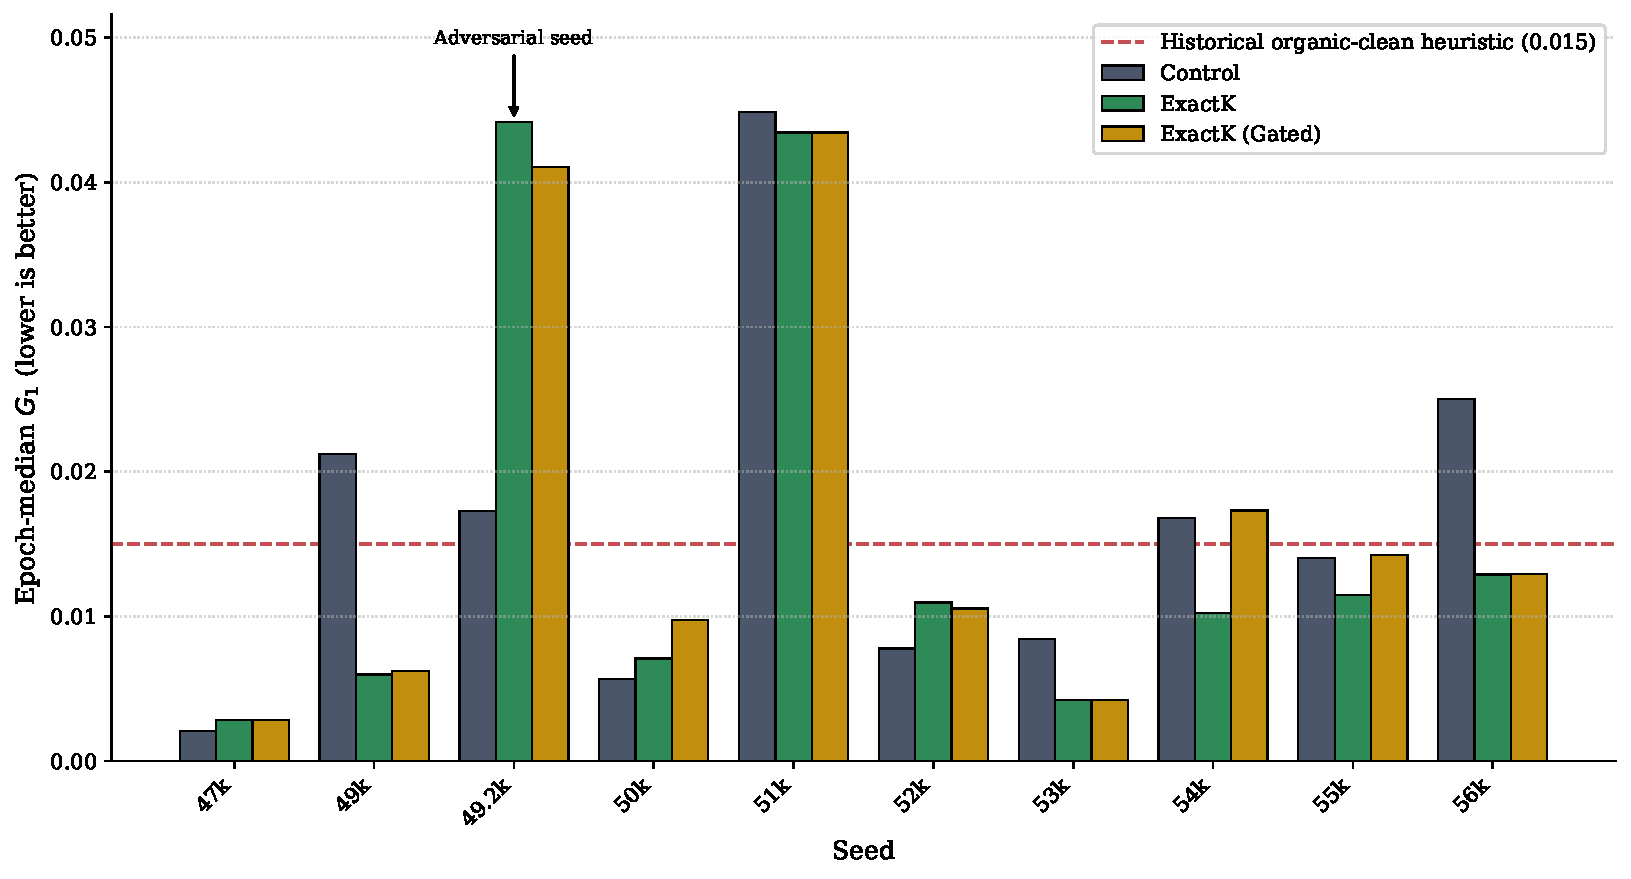
\includegraphics[width=0.75\textwidth]{figure_3_d5.pdf}
\caption{Per-seed epoch-median $G_1$ values for Control, ExactK, and ExactK (Gated) at $d{=}5$, highlighting seed~49200 as the canonical adversarial case in the primary validation suite.}
\label{fig:d5}
\end{figure*}

\subsection{Experiment 2: $d{=}7$ Out-of-Distribution}

To test whether ExactK's hyperparameters transfer across code distances, we ran the identical production configuration at $d{=}7$ ($N_{\text{train}}{=}4096$, $B{=}256$ effective via gradient accumulation, $M{=}512$ max pairs).

\begin{table}[htbp]
\caption{Aggregate results at $d{=}7$ (10~seeds, same hyperparameters as $d{=}5$).}
\label{tab:d7}
\begin{ruledtabular}
\begin{tabular}{llll}
Arm & Median $G_1$ & $\Delta$ vs Control & Topo.\ collapses \\
\hline
Control & 0.0274 & --- & 0/10 \\
\textbf{ExactK} & \textbf{0.0210} & \textbf{+23.4\%} & \textbf{0/10} \\
ExactK EarlyCutoff & 0.0260 & +5.1\% & 0/10 \\
\end{tabular}
\end{ruledtabular}
\end{table}

The $d{=}5$ hyperparameters transfer to $d{=}7$ without modification, achieving a $23.4\%$ $G_1$ reduction (paired bootstrap 95\% CI: $[-51.4\%, 51.4\%]$), which still exceeds the pre-specified $20\%$ out-of-distribution threshold at the point-estimate level. The regression from $31.2\%$ to $23.4\%$ may reflect the substantially larger representation space at $d{=}7$ (336 vs 120~detectors) and other scaling-related factors; we do not claim a definitive explanation.

Seed-level adversariality proved distance-dependent (Fig.~\ref{fig:d7}): seed~49200 was strongly adversarial at $d{=}5$ ($-155.6\%$) but beneficial at $d{=}7$ ($+60.8\%$). Conversely, seeds~51000 ($-40.4\%$) and 55000 ($-584.1\%$) were adversarial at $d{=}7$ but not at $d{=}5$. The EarlyCutoff arm, which set $\lambda{=}0$ after epoch~8, achieved only $+5.1\%$---the hard cutoff removed useful late-epoch ranking signal that the gradual decay ($0.85^{(\text{ep}-8)}$) preserves.

Alignment: $360/360$ PASS. Zero topology collapses. No NaN/Inf.

\begin{figure*}
\centering
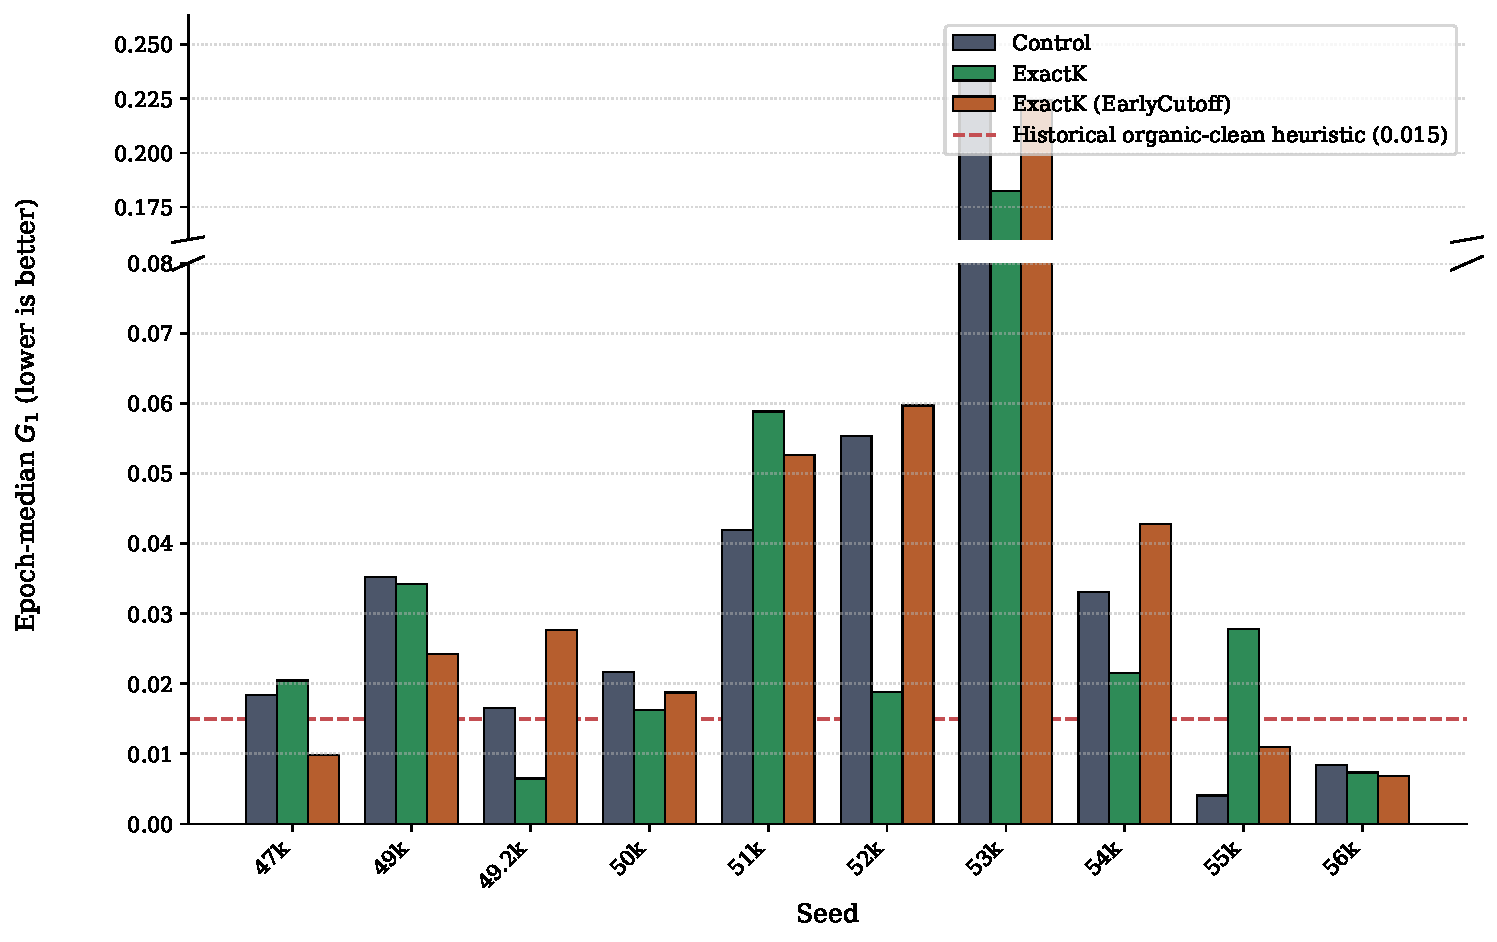
\includegraphics[width=0.75\textwidth]{figure_4_d7_broken_axis.pdf}
\caption{Per-seed epoch-median $G_1$ values for Control, ExactK, and ExactK (EarlyCutoff) at $d{=}7$. A broken $y$-axis is used to preserve visibility of non-outlier seeds while retaining the large 53k outlier in the same panel.}
\label{fig:d7}
\end{figure*}

\subsection{Experiment 3: Holdout Validation}

We evaluated ExactK on 10~holdout seeds ($60000$--$60009$) that were never used during any development iteration, at $d{=}7$, $p{=}0.04$.

\begin{table}[htbp]
\caption{Holdout KPIs (unseen seeds, $d{=}7$).}
\label{tab:holdout}
\begin{ruledtabular}
\begin{tabular}{llll}
KPI & Value & Target & Status \\
\hline
Science $\Delta$ (epoch-median $G_1$) & $+45.0\%$ & $\geq 20\%$ & Pass \\
Safe Yield (Prod CLEAN) & 80\% (8/10) & $\geq 80\%$ & Pass \\
TOPO\_FAIL & 0/10 & $\leq 10\%$ & Pass \\
KPI-B: Leaky cohort & $+15.1\%$ (83\% wins) & $> 0$ & Pass \\
Do-No-Harm violations & 0 & 0 & Pass \\
Max spike $\delta$ (CLEAN) & 0.0063 & $< 0.015$ & Pass \\
\end{tabular}
\end{ruledtabular}
\end{table}

The canonical holdout epoch-median medians are $0.035585$ for Control and $0.019559$ for ExactK, corresponding to a $+45.0\%$ science delta (Fig.~\ref{fig:holdout}). A paired bootstrap over the 10~holdout seed pairs gives a 95\% CI of $[-31.9\%, 60.7\%]$. Because the holdout seeds were reserved throughout development, this result substantially reduces concern about seed-selection bias. However, it validates within the same physical regime ($d{=}7$, $p{=}0.04$, $X$~basis, correlated crosstalk noise). The canonical Day~75 result was produced in the validated reference environment documented by the project reproduction policy. A separate cross-platform reproduction run on different hardware produced a smaller $+12.4\%$ science delta, while preserving the core safety conclusions (zero topology collapses, 240/240 alignment checks passing, and zero Do-No-Harm violations); the selector-oriented deployment KPIs also shifted numerically across environments (for example, safe yield changed from the canonical 80\% to 90\% in that reproduction). We therefore treat the Day~75 canonical tables as the authoritative point estimates for the paper and the reproduction run as a robustness check on directional efficacy and safety rather than as a replacement source of headline numbers. Cross-regime generalization---to other error rates, noise models, bases, or code distances beyond $d{=}7$---remains untested.

Alignment: $240/240$ PASS. Zero topology collapses. No NaN/Inf.

\begin{figure*}
\centering
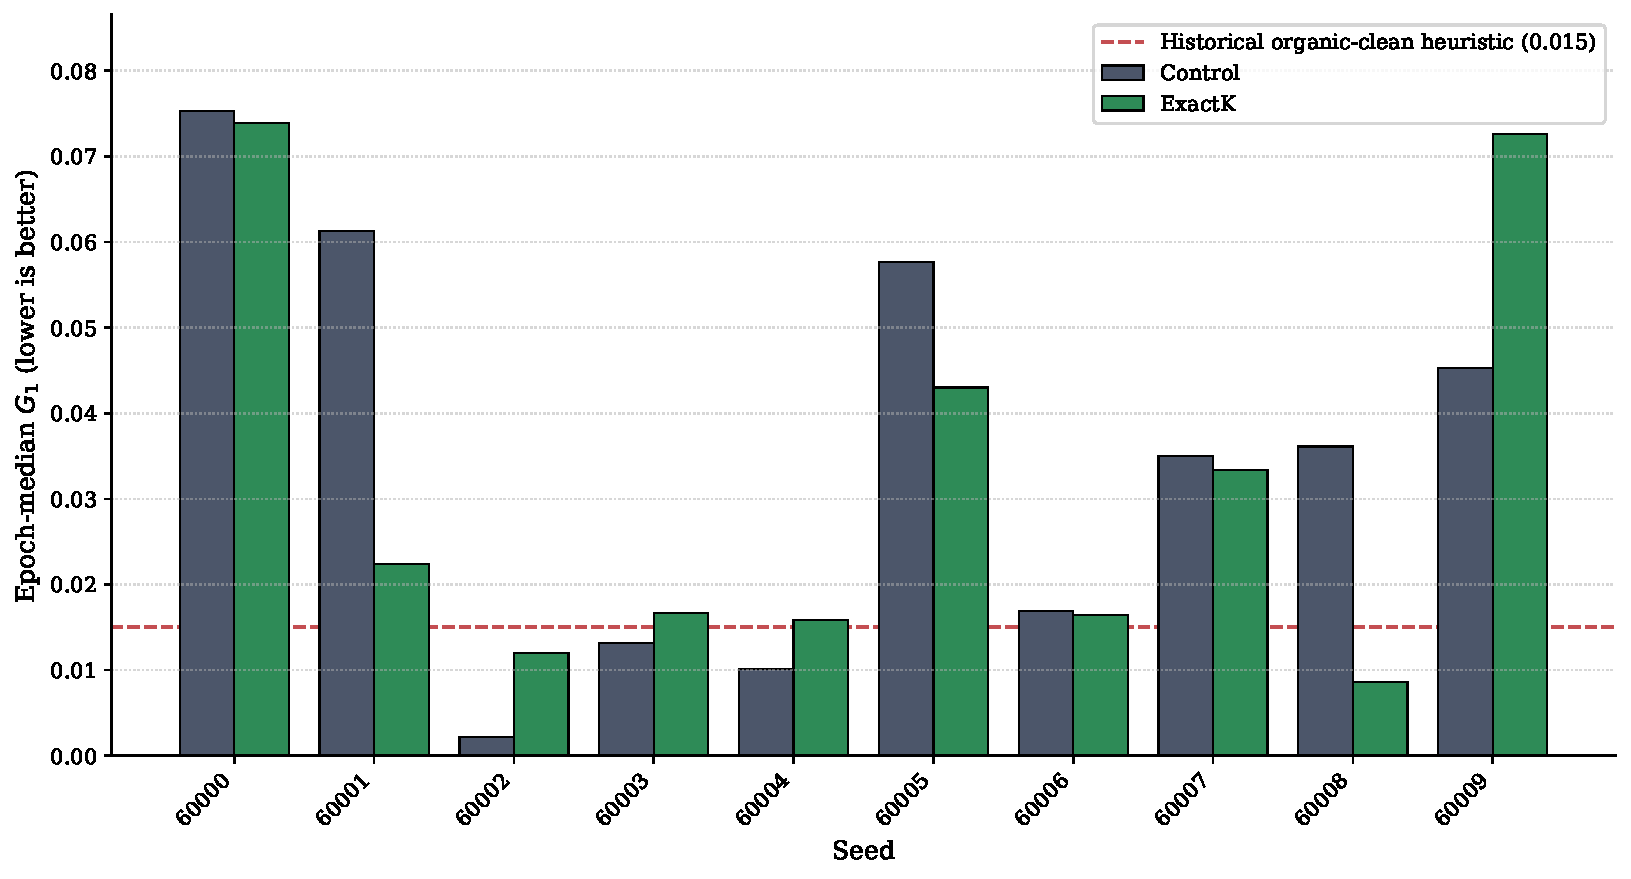
\includegraphics[width=0.75\textwidth]{figure_5_holdout.pdf}
\caption{Per-seed epoch-median $G_1$ values for the unseen holdout seeds 60000--60009 under Control and ExactK.}
\label{fig:holdout}
\end{figure*}

\subsection{Ablation: ExactK vs NearK}
\label{sec:ablation_dk}

This ablation tests the necessity of exact $K$ matching ($\Delta K{=}0$) against the relaxed variant ($|\Delta K| \leq 1$), which yields more pairs per batch but reintroduces inter-bin density confounding.

\begin{table}[htbp]
\caption{$\Delta K$ ablation (4~hard seeds, $d{=}5$, $N_{\text{train}}{=}2048$).}
\label{tab:ablation_dk}
\begin{ruledtabular}
\begin{tabular}{lllll}
Arm & $\Delta K$ & Median $G_1$ & $\Delta$ vs Control & Topology \\
\hline
Control & --- & 0.0224 & --- & OK \\
ExactK & 0 & 0.0112 & $+50.0\%$ & OK (all seeds) \\
NearK & 1 & 0.0573 & $-155.0\%$ (worse) & Collapse (seed 53k) \\
\end{tabular}
\end{ruledtabular}
\end{table}

NearK not only failed to improve over control but dramatically increased leakage and caused topology collapse on seed~53000. The result confirms that adjacent-$K$ pairing reintroduces density confounding: the model can satisfy the hinge margin on $\Delta K{=}1$ pairs by exploiting the systematic error-rate difference between adjacent bins rather than learning spatial topology.

\subsection{Ablation: Margin and Decay Schedule}
\label{sec:ablation_margin}

\begin{table}[htbp]
\caption{Margin calibration ($d{=}5$, $N_{\text{train}}{=}2048$, 10~seeds).}
\label{tab:ablation_margin}
\begin{ruledtabular}
\begin{tabular}{llll}
Configuration & Margin & Decay & Median $G_1$ $\Delta$ \\
\hline
Day 68 (Base) & 0.50 & None & $+26.6\%$ \\
Day 69 (Tuned) & 0.30 & $0.85^{(\text{ep}-8)}$ & $+31.2\%$ \\
\end{tabular}
\end{ruledtabular}
\end{table}

Reducing the margin from $0.50$ to $0.30$ appears to have been the primary driver, increasing the median improvement by approximately 5~percentage points. The $\lambda$ decay schedule appears to have contributed additional late-epoch stability by reducing ranking pressure after epoch~8. Both hyperparameters were hand-tuned for $d{=}5$, $p{=}0.04$.

\subsection{Safety Invariants}

\begin{table}[htbp]
\caption{Safety summary across all ExactK experiments.}
\label{tab:safety}
\begin{ruledtabular}
\begin{tabular}{lllll}
Experiment & Alignment & Topo.\ collapses & NaN/Inf & Seeds \\
\hline
$d{=}5$ (Day 69) & 360/360 & 0 & 0 & 10 \\
$d{=}7$ OOD (Day 70) & 360/360 & 0 & 0 & 10 \\
Holdout (Day 75) & 240/240 & 0 & 0 & 10 \\
\textbf{Total} & \textbf{960/960} & \textbf{0} & \textbf{0} & \textbf{30} \\
\end{tabular}
\end{ruledtabular}
\end{table}

% ══════════════════════════════════════════════════════════════════════
% Section 5: Checkpoint Selection
% ══════════════════════════════════════════════════════════════════════

\section{Checkpoint Selection and the Asymmetric Selection Paradox}
\label{sec:selector}

\subsection{The Problem}

Epoch-median $G_1$ measures treatment efficacy in aggregate but is not a deployment-time object: deploying a decoder requires selecting a \emph{single checkpoint} per trained model. Naive strategies such as selecting the epoch with minimum $G_1$ cherry-pick noise dips---epochs where $G_1$ happens to be near zero---causing both arms to converge to indistinguishable values and destroying the measured treatment effect. This is a general hazard for any per-epoch selection criterion applied to noisy training trajectories.

\subsection{The Asymmetric Selection Paradox}

The holdout experiment (Day~75) revealed a subtle metric failure. Our checkpoint selector (v6) assigns each seed-epoch to one of two pools based on leakage level:

\begin{itemize}
\item \textbf{CLEAN pool} (epochs satisfying dual-cap thresholds on rolling $G_1$): selection objective is $\arg\max(\mathrm{tg\_roll})$---maximize topology quality.
\item \textbf{LEAKY pool} (surviving epochs not in CLEAN): selection objective is $\arg\min(\mathrm{g1\_roll})$---minimize leakage.
\end{itemize}

Because these pools optimize different objectives, comparing the \emph{selected} $G_1$ between arms is invalid when the arms are routed to different pools. In the holdout, control often selected LEAKY-pool epochs with near-zero $\mathrm{g1\_roll}$, while ExactK selected CLEAN-pool epochs optimized for topology rather than minimum~$G_1$. The resulting ``deployment $\Delta$'' of $-324.8\%$ was a metric artifact, not a physics failure.

We term this the \emph{Asymmetric Selection Paradox}: any multi-objective selector with heterogeneous pool criteria produces incomparable inter-arm metrics unless the comparison is restricted to the shared objective. Our resolution is to permanently deprecate selected-$G_1$ comparisons and to evaluate treatment efficacy via epoch-median~$G_1$ (which aggregates over all active epochs regardless of selector routing). Deployment readiness is instead assessed through Safe Yield (fraction of seeds in the CLEAN pool), TOPO\_FAIL rate, and Do-No-Harm constraints.

\subsection{Selector v6}

The production selector uses a single survival filter ($\mathrm{tg\_roll} \geq -0.015$) and the following pool structure:

\begin{table*}
\caption{Selector v6 pool structure.}
\renewcommand{\arraystretch}{1.25}
\begin{ruledtabular}
\begin{tabular}{lll}
Pool & Entry criteria & Selection objective \\
\hline
CLEAN & $\mathrm{g1\_roll} \leq 0.025$ and $\mathrm{g1\_aligned} \leq 0.035$ & $\arg\max(\mathrm{tg\_roll})$; tie-break: lower $\mathrm{g1\_roll}$ \\[2pt]
LEAKY & Surviving, not CLEAN & $\arg\min(\mathrm{g1\_roll})$; tie-break: higher $\mathrm{tg\_roll}$ \\[2pt]
TOPO\_FAIL & No surviving epochs & $\arg\max(\mathrm{tg\_roll})$; tie-break: lower $\mathrm{g1\_roll}$ \\
\end{tabular}
\end{ruledtabular}
\renewcommand{\arraystretch}{1.0}
\end{table*}

Rolling metrics ($\mathrm{g1\_roll}$, $\mathrm{tg\_roll}$) use a trailing median window of 3~epochs. The dual-cap qualification for CLEAN requires both rolling $G_1$ and the aligned instantaneous check $\mathrm{G1\_aligned}$ to remain below threshold, preventing selection of epochs where the rolling median is low but a single-epoch spike violates the bound. Full pseudo-code and the selector evolution from v1 through v6 are provided in Appendix~\ref{app:selector}. Implementation details (JSONL write-ahead logging, progressive checkpointing, receipt schema) are in Appendix~\ref{app:impl}.

% ══════════════════════════════════════════════════════════════════════
% Section 6: Related Work
% ══════════════════════════════════════════════════════════════════════

\section{Related Work}

\paragraph{ML decoders for QEC.} Neural approaches to surface-code decoding include feedforward networks~\cite{PLACEHOLDER_mlp_decoder}, graph neural networks~\cite{PLACEHOLDER_gnn_decoder}, recurrent architectures~\cite{PLACEHOLDER_rnn_decoder}, and transformers~\cite{PLACEHOLDER_transformer_decoder}. These works focus primarily on decoder \emph{accuracy}---matching or exceeding MWPM---rather than on \emph{training methodology}. Our contribution is orthogonal: ExactK addresses a training-time confound (K-leakage) that affects any neural decoder whose internal representation can encode syndrome count, regardless of architecture. We do not claim that the factor-graph decoder used in this study outperforms MWPM at the final configuration; this comparison was not performed.

\paragraph{Factor-graph and BP-inspired decoders.} Belief-propagation decoders and their neural extensions have been applied to classical LDPC codes~\cite{PLACEHOLDER_bp_neural} and, more recently, to quantum codes~\cite{PLACEHOLDER_bp_quantum}. Our bipartite factor-graph architecture differs in that it preserves the DEM's $k{>}2$ hyperedge structure without clique expansion, and in that its readout pools only error nodes associated with the logical observable.

\paragraph{Shortcut learning and debiasing.} The phenomenon of models exploiting spurious correlations is well documented in the broader ML literature~\cite{PLACEHOLDER_shortcut_learning}. Group distributionally robust optimization (DRO)~\cite{PLACEHOLDER_group_dro} addresses spurious correlations by reweighting or resampling groups. ExactK shares the philosophy of within-group comparison but differs in a critical respect: in QEC, the ``group variable''~$K$ is \emph{physically meaningful}, not purely spurious. Global debiasing methods that treat $K$ as a nuisance variable destroy legitimate signal (Sec.~\ref{sec:prior_mitigation}). ExactK's design---constraining only the auxiliary ranking loss to same-$K$ pairs while leaving the main loss unrestricted---is specific to this partially-legitimate-correlation structure.

\paragraph{Pairwise ranking losses.} Hinge-based ranking losses have a long history in learning-to-rank~\cite{PLACEHOLDER_ranknet} and metric learning~\cite{PLACEHOLDER_contrastive}. ExactK applies constrained pair mining (same-$K$, opposite-label) to a debiasing objective rather than a ranking-quality objective. The constraint $\Delta K{=}0$ is the key distinguishing feature; without it, the mechanism degrades to a form of global decorrelation that fails for the reasons described in Sec.~\ref{sec:prior_mitigation}.

% ══════════════════════════════════════════════════════════════════════
% Section 7: Discussion
% ══════════════════════════════════════════════════════════════════════

\section{Discussion}

\subsection{Why ExactK Succeeded Where Others Failed}

The 14~failed mechanisms (Table~\ref{tab:families}) share a common thread: each operates on the \emph{global} relationship between $z$ and $K$, either by penalizing it (decorrelation, adversarial training), by subtracting it (orthogonalization), by blocking its gradient (shielding), or by routing it to a separate channel (factorization). All of these require distinguishing between legitimate and shortcut $K$-dependence in~$z$---a distinction that cannot be made from the signal alone, because the same covariance structure encodes both.

ExactK avoids this problem entirely by never operating on the global $z$--$K$ relationship. Instead, it constrains only a narrow auxiliary channel---pairwise ranking within iso-$K$ groups---where $K$ is constant and therefore cannot contribute to the ranking signal by construction. The main loss remains free to learn whatever $K$-dependent features are useful for accuracy; ExactK provides a countervailing pressure that encourages the topology channel to carry spatial information rather than density shortcuts.

The specific failure modes of each family are instructive:
\begin{itemize}
\item \textbf{Global regularization} cannot distinguish physics from shortcut: $\Corr(z, K)^2$ penalizes both. With hysteresis gating, the penalty is safe but too weak ($+13.6\%$).
\item \textbf{K-orthogonalization} suffers from the bootstrap problem: $\beta$ must be estimated from the same data it corrects. Per-batch estimates are too noisy at $B{=}64$--$128$; cross-epoch estimates become stale as the model updates.
\item \textbf{Gradient shielding} removes the $K$-collinear gradient component, which on a substantial subset of tested seeds also carries genuine topology signal. Reducing the projection strength ($\lambda{=}1.0 \to 0.25$) does not resolve the issue.
\item \textbf{Nuisance siphon} was architecturally inert: both output channels became equally uncorrelated with~$K$. The observed improvement was attributable to the decorrelation regularizer, confirming that the factorization added no value.
\end{itemize}

\subsection{The Adversarial Seed Phenomenon}
\label{sec:adversarial}

A minority of seeds showed increased $G_1$ under ExactK, with the exact fraction varying across experiments. Notably, adversarial behavior is distance-dependent: seed~49200 was strongly adversarial at $d{=}5$ ($-155.6\%$) but beneficial at $d{=}7$ ($+60.8\%$). Seeds~51000 and 55000 showed the reverse pattern.

One plausible interpretation is that in the lower-dimensional $d{=}5$ setting (120~detectors), the strict iso-$K$ constraint may conflict more directly with seed-specific topology structure, leaving fewer representational degrees of freedom to satisfy both the main loss and the auxiliary ranking. In the larger $d{=}7$ setting (336~detectors), the higher-dimensional representation may offer more flexibility for accommodating the iso-$K$ ranking constraint without topology damage. We emphasize that this is a hypothesis consistent with the observed reversal, not an established mechanism.

Two reactive guards were tested: StopOnRise (freeze $\lambda{=}0$ upon detecting a $G_1$ spike) and RatioCapped (cap the iso-$K$/focal loss ratio at $20\%$). Neither improved the adversarial seed without damaging winning seeds. The production policy accepts the adversarial minority as the cost of the median improvement.

\subsection{Limitations}

\paragraph{Tested regime.} All experiments used a single noise model (correlated crosstalk, $c{=}0.5$), a single physical error rate ($p{=}0.04$), a single basis ($X$), and two code distances ($d{=}5$, $d{=}7$). Generalization to other noise models (e.g., SI1000-like, biased-$Z$, real hardware noise), other error rates, other bases, and larger code distances ($d \geq 9$) has not been validated.

\paragraph{Statistical power.} The main validation suites use 10~seeds each, while the Day~67 $\Delta K$ ablation uses 4~hard seeds. Paired bootstrap 95\% CIs for the median improvement are consequently wide and span zero even when the point estimates are large ($d{=}5$: $31.2\%$, paired bootstrap 95\% CI $[-46.3\%, 61.2\%]$; $d{=}7$: $23.4\%$, paired bootstrap 95\% CI $[-51.4\%, 51.4\%]$; holdout: $45.0\%$, paired bootstrap 95\% CI $[-31.9\%, 60.7\%]$). This reflects genuine seed heterogeneity and the presence of adversarial seeds, and it limits how strongly any single-regime quantitative estimate should be generalized.

\paragraph{Linear leakage only.} $G_1$ measures linear $K$-leakage. Nonlinear leakage was detected by early diagnostics but is neither targeted by ExactK nor measured by~$G_1$. The reported improvements therefore reflect reduction of the dominant linear leakage mode.

\paragraph{No MWPM comparison at final configuration.} The paper does not claim that the ExactK-trained factor-graph decoder outperforms MWPM\@. The MWPM benchmarks conducted earlier in the project used a different model (GNN v1), and no comparison was performed at the final factor-graph + ExactK configuration.

\paragraph{Hyperparameter transfer.} The margin ($m{=}0.30$), loss weight ($\lambda{=}0.10$), and decay schedule ($0.85^{(\text{ep}-8)}$) were hand-tuned for $d{=}5$, $p{=}0.04$. These transferred to $d{=}7$ without modification, but transfer to substantially different regimes ($d{=}9$, $p{=}0.01$) is untested.

\paragraph{Hardware reproducibility.} The $d{=}5$ canonical results were produced on CPU in the local development environment, whereas the $d{=}7$/holdout canonical results were produced on GPU in the validated RunPod environment. Cross-platform reproduction is expected to preserve qualitative conclusions and safety invariants while allowing numerically different point estimates.

\subsection{Future Work}

Several directions follow from this work: (i)~cross-$p$ validation to test whether the production hyperparameters transfer across physical error rates; (ii)~evaluation at larger code distances ($d{=}9$, $d{=}11$) with adapted pair budgets; (iii)~validation on diverse noise models including SI1000-like and empirical hardware noise profiles; (iv)~development of pre-training diagnostics (e.g., DEM graph features) to predict seed-level compatibility with ExactK; (v)~adaptive $\lambda$ scheduling based on online $G_1$ monitoring; (vi)~formal analysis of the relationship between $\Delta K{=}0$ pair mining and gradient-level $K$-independence under the auxiliary loss.

% ══════════════════════════════════════════════════════════════════════
% Section 8: Conclusion
% ══════════════════════════════════════════════════════════════════════

\section{Conclusion}

We introduced ExactK, an iso-$K$ hinge loss that removes within-pair $K$ variation from the auxiliary ranking objective in QEC neural decoder training. The mechanism is minimal---a pair-mining step within each batch---and operates entirely in the forward pass, requiring no gradient surgery, no architectural modification, and no adversarial training.

The design of ExactK was motivated by a systematic evaluation of 14~prior mechanisms across five families, all of which failed to reliably reduce K-leakage while preserving topology signal across seeds at the required effect size. The common failure mode was that syndrome count~$K$ carries physically meaningful information in QEC, so interventions targeting global $z$--$K$ dependence inevitably destroy legitimate covariance alongside shortcuts. ExactK sidesteps this by constraining only within-$K$ comparisons in the auxiliary loss.

In the tested regime---surface codes at $d{=}5$ and $d{=}7$ with correlated crosstalk noise at $p{=}0.04$---ExactK reduced linear K-leakage ($G_1$) by $31.2\%$ at $d{=}5$, $23.4\%$ at $d{=}7$ using the same hyperparameters, and $45.0\%$ on unseen holdout seeds, with zero topology collapses across the 30-seed Day~69/70/75 validation suite and 960/960 alignment checks passing. A minority of seeds showed increased leakage---an adversarial subset whose behavior is distance-dependent and, at present, unpredictable.

These results indicate that K-leakage in neural QEC decoders can be substantially reduced through targeted within-$K$ ranking pressure, and that the strict $\Delta K{=}0$ constraint is essential---relaxing to $\Delta K{=}1$ reintroduces the confounding it is designed to remove. The mechanism's simplicity makes it a practical candidate for integration into QEC decoder training pipelines, subject to validation across a broader range of physical regimes.

% ══════════════════════════════════════════════════════════════════════
% End Matter: Acknowledgements, Funding, COI, Author Contributions,
%             AI Disclosure, Data Availability
% ══════════════════════════════════════════════════════════════════════

\section*{Acknowledgements}

The author thanks the open-source maintainers of Stim, PyMatching, and PyTorch for the infrastructure on which this work was built.

\section*{Funding}

This work received no external funding.

\section*{Competing Interests}

The author declares no competing interests.

\section*{Author Contributions}

Mohammad Albataineh directed the overall project workflow, selected and prioritized research directions, reviewed and validated experimental outputs, integrated the final manuscript and release artifacts, and approved the final version. Large language model tools were used extensively for coding assistance, debugging, drafting, editing, formatting, and document preparation.

\section*{AI Assistance Disclosure}

This work was developed through a heavily AI-assisted workflow. Large language model tools were used extensively across research planning support, experiment orchestration, code generation and revision, debugging, manuscript drafting and editing, and \LaTeX/PDF preparation. The author's role was to direct and manage the workflow, review generated material, validate the final outputs used in the paper, integrate the final manuscript and project artifacts, and assume full responsibility for the scientific claims, reported results, and interpretations.

\section*{Data and Code Availability}

The code, experiment artifacts, and reproduction scripts associated with this work are contained in the project repository and release bundle. Public access details will be provided at publication time.

% ══════════════════════════════════════════════════════════════════════
% Appendices A–D
% ══════════════════════════════════════════════════════════════════════

\appendix

% ──────────────────────────────────────────────────────────────────────
\section{Detailed Negative Results}
\label{app:negative}

The following expands Table~\ref{tab:families} with per-mechanism development-day references and specific failure observations. The 14~mechanisms are grouped into the five canonical families. Mechanism numbering below follows development chronology within each family.

\subsection{Global Regularization / Decorrelation (3 mechanisms)}

\paragraph{Mechanism 1 --- GRL adversary (Days 44--45).} A gradient reversal layer was applied to the $z$ representation to adversarially remove $K$-information. At the original GRL strength (Day~44), the adversarial pressure caused topology collapse: $\overline{\SliceC} = 0.451$, indistinguishable from random (${\sim}0.50$). Reducing the GRL $\lambda$ (Day~45) preserved topology ($\TG = +0.026$) but failed to achieve a reliable topology--leakage tradeoff: $G_1 = 0.035$ remained comparable to the control baseline. At no tested $\lambda$ did the GRL simultaneously preserve topology and reduce leakage below control.

\paragraph{Mechanism 2 --- $\Corr(z, K)^2$ leakage penalty (Day 46).} A squared Pearson correlation penalty was added to the training loss. The penalty term diverged in magnitude: the scrambler norm reached $\|\mathrm{scr}\| = 2.1$ versus control $0.06$, indicating the loss amplified rather than suppressed the $K$-correlated component.

\paragraph{Mechanism 3 --- Decorrelation with hysteresis gating (Day 66).} A refined version of the correlation penalty, gated by a hysteresis controller that activated the penalty only when $|\Corr(z, K)|$ exceeded a threshold. The gating made the mechanism safe (zero topology collapses) but underpowered: $+13.6\%$ median $G_1$ reduction, below the $30\%$ PASS threshold.

\subsection{Null-Space Alignment (4 mechanisms)}

\paragraph{Mechanism 4 --- Null-space + multi-gate pipeline (Day 47).} A loss encouraging the residual to lie in the null space of~$K$, combined with a pipeline of 6~gate conditions (G1--G6). Achieved 5/6 passes on seed~47000 but failed G4 ($\|\mathrm{scr}\| = 0.20 > 0.10$ threshold) and failed outright on seeds~49000 and 49200. The mechanism was fundamentally seed-dependent.

\paragraph{Mechanism 5 --- Normalizer gaming fix (Day 48).} The Day~47 pipeline was found to have a normalizer gaming exploit: applying KCS to the scrambled residual introduced a systematic $-1.0$ offset (because $\mu_K[\text{bin}]$ is computed on the unscrambled data). Reverting to raw~$z$ for the null-space loss fixed the offset but rendered the null-space mechanism inert.

\paragraph{Mechanism 6 --- Bias-free head + EMA centering (Day 49).} Removing all bias terms and replacing batch normalization with EMA-based centering caused catastrophic $\tanh$ saturation: the scrambler norm exploded to $36$--$297$, rendering the model non-functional.

\paragraph{Mechanism 7 --- Baseline-centered null-space (Day 50).} A centering scheme subtracting the per-$K$-bin baseline from~$z$ before computing the null-space loss. Achieved 6/6 gates on seed~47000 but failed on seeds~49000 and 49200 with the same configuration. The root cause was that the optimal centering offset was seed-specific.

\subsection{K-Orthogonalization (5 mechanisms)}

\paragraph{Mechanism 8 --- Controller-based $\sigma$-EMA phases (Days 51--54).} An adaptive controller governed the $\lambda$ schedule for K-correction based on an EMA of the residual standard deviation. The controller entered a failure loop: $\sigma \to \sigma_{\mathrm{floor}}$ (sigma collapse), followed by $G_1$ oscillation between $0$ and $0.6$ as the controller alternated between aggressive and passive phases. No stable operating point was found across 4~iterations.

\paragraph{Mechanism 9 --- Per-batch OLS K-orthogonalization (Day 56).} The linear regression coefficient $\beta$ (regressing $z$ on $K$) was estimated per batch and subtracted: $z' = z - \beta K$. At batch size $B{=}64$, the $\beta$ estimate was catastrophically noisy: $\beta = 129$ on one batch, causing loss $= 1.0 \times 10^{160}$ and numerical divergence.

\paragraph{Mechanism 10 --- Safeguarded K-ortho (Day 57).} Caps ($|\beta| \leq 1.0$), floors ($\sigma_K \geq 0.1$), and an activity gate ($|\hat{r}| \geq 0.05$) were added to prevent divergence. The gate was too restrictive: $27\%$ of epochs were classified as NO\_OP ($\beta \approx 0.002$), and the active epochs produced negligible correction.

\paragraph{Mechanism 11 --- EMA cross-epoch K-ortho with global gate (Day 58).} A global activity gate required $R^2_{\mathrm{global}} \geq 0.10$ before applying any correction. The global $R^2$ hovered at ${\sim}0.01$---well below threshold---because the density-residual decomposition had already removed most of the coarse $K$-dependence. The gate never opened; $100\%$ of epochs were NO\_OP.

\paragraph{Mechanism 12 --- Frozen $\beta$ from OrthoStatSet (Day 59).} A dedicated calibration dataset (OrthoStatSet) was used to estimate $\beta$ once before training, then frozen. The frozen estimate became stale as the model's representation drifted during training. $G_1$ worsened by $-56\%$ relative to control.

\subsection{Gradient Shielding (1 mechanism, 3 strength variants)}

\paragraph{Mechanism 13 --- Hard/soft/adaptive gradient shielding (Days 62--64).} The $K$-collinear component of the loss gradient was projected out before the optimizer step: $g' = g - \frac{g \cdot g_K}{\|g_K\|^2} g_K$. Three projection strengths were tested ($\lambda = 1.0$, $0.5$, $0.25$). All three caused topology collapse on seed~53000. The mechanism failed because the $K$-collinear gradient component carried genuine topology information on a substantial fraction of the tested seeds: removing it ablated legitimate spatial gradient alongside the leakage component.

A softer variant---weighting the projection by the estimated $K$-leakage severity---achieved $+59.3\%$ on 3~favorable seeds but $-54.2\%$ on the full 10-seed suite, confirming that the problem was structural rather than a matter of calibration.

\subsection{Architectural Factorization (1 mechanism)}

\paragraph{Mechanism 14 --- Split residual head + nuisance siphon (Day 65).} The residual head was split into two output channels: a topology channel and a nuisance siphon intended to absorb $K$-dependent signal. When combined with a decorrelation regularizer, the configuration achieved $+29.9\%$ median $G_1$ reduction but with topology collapse on 1 of the tested seeds. Post-hoc analysis revealed that the siphon channel was architecturally inert---both channels became equally uncorrelated with~$K$. The observed improvement was attributable to the accompanying decorrelation regularizer (see Mechanism~3 above), confirming that the factorization itself added no value.

% ──────────────────────────────────────────────────────────────────────
\onecolumngrid
\section{Checkpoint Selector Pseudo-Code and Evolution}
\label{app:selector}

\subsection{Selector v6 Pseudo-Code}

\begin{lstlisting}
FUNCTION SelectEpoch(metrics_by_epoch, params):
    INPUT:
        metrics_by_epoch: list of {epoch, G1_aligned, topo_TG, slice_clean, ...}
        params:
            tau_clean     = 0.025   # g1_roll cap for CLEAN pool
            tau_clean_hi  = 0.035   # g1_aligned instantaneous cap
            tg_floor      = -0.015  # minimum tg_roll for survival
            active_min    = 6       # skip warmup epochs 1-5
            roll_window   = 3       # trailing median window

    1. FILTER active epochs: active = {e in metrics | e.epoch >= active_min}

    2. COMPUTE rolling medians (trailing window = 3):
         g1_roll[e]  = median(G1_aligned over [e-2, e-1, e])
         tg_roll[e]  = median(topo_TG  over [e-2, e-1, e])
         sc_roll[e]  = median(slice_clean over [e-2, e-1, e])

    3. SURVIVAL filter:
         surviving = {e in active | tg_roll[e] >= tg_floor}
         # In production (drop_slice_floor=True), skip sc_roll check

    4. POOL assignment:
         clean_pool = {e in surviving |
                       g1_roll[e] <= tau_clean AND
                       e.G1_aligned <= tau_clean_hi}
         leaky_pool = surviving \ clean_pool

    5. SELECTION:
         IF surviving is empty:
             mode = TOPO_FAIL
             chosen = argmax(tg_roll) over active
             tie-break: lower g1_roll
         ELIF clean_pool is non-empty:
             mode = CLEAN_MAX_TG
             chosen = argmax(tg_roll) over clean_pool
             tie-break: higher sc_roll, then lower g1_roll
         ELSE:
             mode = LEAKY_MIN_G1ROLL
             chosen = argmin(g1_roll) over surviving
             tie-break: higher tg_roll

    RETURN {chosen_epoch, mode, g1_roll, tg_roll, sc_roll,
            n_active, n_surviving, n_clean, n_leaky}
\end{lstlisting}

\subsection{Selector Evolution}

The checkpoint selector underwent six iterations driven by empirical failures at increasing code distance:

\begin{table*}
\caption{Selector version history.}
\label{tab:selector_evolution}
\renewcommand{\arraystretch}{1.2}
\begin{ruledtabular}
\begin{tabular}{llll}
Version & Day & Key change & Failure that motivated it \\
\hline
v1 & 69 & Min-$G_1$ fallback, single threshold & Cherry-picks noise dips in $G_1$ trajectory \\
v2 & 70 & Added SliceClean as secondary check & SliceClean itself too noisy at $d{=}7$ \\
v3 & 71 & SliceClean survival filter (hard floor) & 80\% TOPO\_FAIL rate at $d{=}7$ \\
v4 & 72 & Relaxed SliceClean floor & Same underlying instability \\
v5 & 73a & Rolling medians for $G_1$ (window=3) & Smoothing helped $G_1$ but not SliceClean \\
\textbf{v6} & \textbf{73b} & \textbf{\texttt{drop\_slice\_floor} + dual-cap CLEAN} & \textbf{Eliminates SliceClean survival noise} \\
\end{tabular}
\end{ruledtabular}
\renewcommand{\arraystretch}{1.0}
\end{table*}

The critical insight from v3$\to$v6 was that SliceClean, while useful as a quality metric, was too noisy at $d{=}7$ to serve as a survival filter. The \texttt{drop\_slice\_floor} flag in v6 removes SliceClean from the survival gate while retaining it as a tie-breaker within the CLEAN pool selection. The dual-cap qualification for CLEAN (both $\mathrm{g1\_roll} \leq 0.025$ and $\mathrm{G1\_aligned} \leq 0.035$) prevents selection of epochs where the rolling median is acceptably low but a single-epoch $G_1$ spike violates the bound.

\subsection{Dual-Cap Rationale}

The CLEAN pool uses two separate $G_1$ thresholds:

\begin{enumerate}
\item \textbf{Rolling cap} ($\mathrm{g1\_roll} \leq 0.025$): ensures the trailing trend is low, preventing entry based on a single lucky epoch.
\item \textbf{Instantaneous cap} ($\mathrm{G1\_aligned} \leq 0.035$): ensures the epoch being considered does not itself have an anomalously high $G_1$ that would be masked by the rolling median.
\end{enumerate}

Both must be satisfied for CLEAN qualification. This addresses a failure mode observed in v5 where an epoch with $G_1 = 0.08$ qualified for CLEAN because its rolling median (dragged down by two preceding low-$G_1$ epochs) was below $0.025$.
\twocolumngrid

% ──────────────────────────────────────────────────────────────────────
\section{Cross-Platform Reproduction}
\label{app:repro}

\subsection{Reference Environments}

All canonical results in this paper were produced in one of two validated environments:

\begin{table*}
\caption{Reference environments.}
\label{tab:environments}
\begin{ruledtabular}
\begin{tabular}{lllll}
Label & Platform & OS & Hardware & Used for \\
\hline
\textbf{DEV} & Local workstation & Windows 11 & Intel i7-14700HX, CPU-only & $d{=}5$ canonical (Day 69) \\
\textbf{GPU} & RunPod cloud & Ubuntu 24.04 (Docker) & NVIDIA RTX PRO 6000 (96\,GB) & $d{=}7$ canonical (Day 70), holdout (Day 75) \\
\end{tabular}
\end{ruledtabular}
\end{table*}

\subsection{Sources of Non-Determinism}

Cross-platform numerical differences arise from:

\begin{enumerate}
\item \textbf{Floating-point non-associativity.} Summation order in scatter-mean operations differs between CPU and GPU backends, and between CUDA kernel implementations. This affects message-passing aggregation and batch-level loss computation.
\item \textbf{cuDNN non-determinism.} Even with \texttt{torch.use\_deterministic\_algorithms(True)}, some operations (e.g., atomic scatter-add on GPU) may remain non-deterministic across runs.
\item \textbf{RNG state divergence.} When the same seed produces different batch orderings due to dataloader threading differences across platforms, the entire training trajectory diverges.
\end{enumerate}

\subsection{Observed Variance}

A cross-platform reproduction of Day~75 (holdout) was conducted on GPU hardware different from the canonical GPU environment:

\begin{table}[htbp]
\caption{Canonical vs.\ reproduction comparison (Day 75 holdout).}
\label{tab:repro}
\begin{ruledtabular}
\begin{tabular}{lll}
Metric & Canonical run & Reproduction run \\
\hline
Science $\Delta$ & $+45.0\%$ & $+12.4\%$ \\
Safe Yield (Prod) & 80\% (8/10) & 90\% (9/10) \\
TOPO\_FAIL & 0/10 & 0/10 \\
Alignment & 240/240 & 240/240 \\
DNH violations & 0 & 0 \\
\end{tabular}
\end{ruledtabular}
\end{table}

The safety invariants (zero topology collapses, full alignment, zero Do-No-Harm violations) were preserved across platforms. The efficacy point estimate ($\Delta$) showed substantial variance ($+45.0\%$ vs $+12.4\%$), consistent with the wide bootstrap confidence intervals reported in Secs.~IV\,B--D and the known sensitivity of the median statistic to individual seed trajectories at $N{=}10$.

\subsection{Reproduction Policy}

The project's reproduction policy treats the canonical results from the validated reference environment as the authoritative point estimates. Cross-platform reproduction is used to validate:

\begin{enumerate}
\item \textbf{Aggregate directional efficacy}: ExactK should improve median $G_1$ relative to control ($\Delta > 0$) in aggregate.
\item \textbf{Safety preservation}: zero topology collapses, full alignment passage, zero Do-No-Harm violations.
\item \textbf{Broad qualitative consistency}: the overall pattern of improvement should be directionally consistent, though individual seed-level responses may vary across platforms.
\end{enumerate}

Exact numerical agreement of point estimates is \emph{not} expected across platforms, and quantitative reproduction targets are not imposed beyond aggregate directional sign consistency.

\subsection{Reproduction Scripts}

Canonical experiment configurations and reproduction scripts are provided in \texttt{scripts/reproduce/}:

\begin{itemize}
\item \texttt{repro\_day69\_d5.sh} --- $d{=}5$ primary validation
\item \texttt{repro\_day70\_d7.sh} --- $d{=}7$ OOD transfer
\item \texttt{repro\_day75\_holdout.sh} --- $d{=}7$ holdout validation
\end{itemize}

Each script specifies the exact seed set, hyperparameters, data generation parameters, and artifact output directory. Running these scripts on a different platform is expected to produce qualitatively consistent aggregate results with numerically different point estimates.

% ──────────────────────────────────────────────────────────────────────
\onecolumngrid
\section{Implementation Details: Logging, Checkpointing, and Receipts}
\label{app:impl}

\subsection{JSONL Write-Ahead Logging}

Each training run produces a per-seed metrics log in JSONL (JSON Lines) format, with one epoch record appended and immediately flushed after each \texttt{log\_epoch()} call. In the canonical production experiment path used for the paper's reported results, the training script additionally calls \texttt{os.fsync()} after \texttt{log\_epoch()}, yielding a write-ahead logging pattern with per-epoch durability guarantees.

\begin{lstlisting}
{"epoch": 1, "loss": 0.6932, "G1_aligned": 0.0412, "topo_TG": 0.031, ...}
{"epoch": 2, "loss": 0.6891, "G1_aligned": 0.0387, "topo_TG": 0.033, ...}
...
\end{lstlisting}

\paragraph{Implementation.} The \texttt{EpochLogger} class opens the log file in append mode and calls \texttt{flush()} after each \texttt{log\_epoch()} invocation. The logger is used as a context manager:

\begin{lstlisting}[language=Python]
with EpochLogger("metrics_47000.jsonl") as logger:
    for epoch in range(1, 13):
        metrics = train_one_epoch(...)
        logger.log_epoch(metrics)
\end{lstlisting}

\paragraph{Core schema.} Each JSONL record contains the following primary fields:

\begin{table*}
\caption{Core JSONL schema fields.}
\begin{ruledtabular}
\begin{tabular}{lll}
Field & Type & Description \\
\hline
\texttt{epoch} & int & 1-indexed epoch number \\
\texttt{loss} & float & Training loss for this epoch \\
\texttt{G1\_aligned} & float & Linear probe $R^2$ ($z \to K$), aligned tensor \\
\texttt{topo\_TG} & float & TopologyGain ($\SliceC_{\text{clean}} - \SliceC_{\text{scrambled}}$) \\
\texttt{slice\_clean} & float & Mean per-$K$-bin AUROC on clean predictions \\
\texttt{mean\_drop} & float & Mean prediction drop under $K$-matched scrambling \\
\end{tabular}
\end{ruledtabular}
\end{table*}

\paragraph{Optional telemetry fields.} Depending on the experiment configuration, records may also include:

\begin{table*}
\caption{Optional telemetry fields.}
\begin{ruledtabular}
\begin{tabular}{lll}
Field & Type & Description \\
\hline
\texttt{G1\_raw\_probe} & float & Raw MLP probe score (historical, pre-Day~55 formats) \\
\texttt{alignment\_ok} & bool & Whether probe tensor matches K-ortho target tensor \\
\texttt{iso\_active} & bool & Whether ExactK loss was active this epoch \\
\texttt{iso\_bce\_ratio} & float & Ratio of ExactK loss to focal loss \\
\texttt{mean\_pairs\_used} & float & Mean number of iso-$K$ pairs mined per batch \\
\texttt{mean\_violation\_rate} & float & Fraction of pairs violating the hinge margin \\
\texttt{mean\_zgap} & float & Mean $z_{\text{pos}} - z_{\text{neg}}$ across mined pairs \\
\texttt{lambda\_epoch} & float & Effective $\lambda$ for this epoch \\
\texttt{nan\_detected} & bool & Whether NaN/Inf was detected in any tensor \\
\end{tabular}
\end{ruledtabular}
\end{table*}

\subsection{Progressive Checkpointing}

Model checkpoints are saved after every epoch as \texttt{ckpt\_\{seed\}\_ep\{epoch\}.pt}, containing the full \texttt{state\_dict}. After selector v6 determines the best epoch for each seed, the pipeline:

\begin{enumerate}
\item Copies the selected checkpoint to \texttt{best\_model\_\{seed\}.pt}.
\item Deletes unselected checkpoints to reclaim disk space.
\end{enumerate}

This progressive strategy avoids the need to choose a checkpoint epoch \emph{during} training while keeping disk usage bounded. The cleanup step is deferred until selector execution is complete, ensuring that the selection decision is never constrained by checkpoint availability.

\subsection{Selection Receipt Schema}

After checkpoint selection, a per-seed JSON receipt is written to \texttt{selection\_receipt\_\{seed\}.json}. The following tables define the paper-facing normalized receipt contract; the raw repository schema may include additional internal fields, but any valid receipt must contain all required fields as populated by the selector's \texttt{\_build\_result} function.

\paragraph{Required fields} (always present in every receipt):

\begin{table*}
\caption{Required receipt fields.}
\begin{ruledtabular}
\begin{tabular}{lll}
Field & Type & Description \\
\hline
\texttt{epoch} & int & Selected epoch \\
\texttt{G1\_aligned} & float & Instantaneous linear probe $R^2$ at selected epoch \\
\texttt{g1\_roll} & float & Trailing-median $G_1$ (window=3) \\
\texttt{g1\_spike\_delta} & float & $\mathrm{G1\_aligned} - \mathrm{g1\_roll}$; positive = spike above trend \\
\texttt{slice\_clean} & float & Per-$K$-bin AUROC at selected epoch \\
\texttt{slice\_clean\_roll} & float & Trailing-median SliceClean \\
\texttt{tg\_roll} & float & Trailing-median TopologyGain \\
\texttt{mean\_drop} & float & Mean prediction drop under scrambling \\
\texttt{selection\_mode} & str & \texttt{CLEAN\_MAX\_TG}, \texttt{LEAKY\_MIN\_G1ROLL}, or \texttt{TOPO\_FAIL\_MAX\_TG} \\
\texttt{n\_active} & int & Epochs passing warmup filter \\
\texttt{n\_surviving} & int & Epochs passing topology-floor survival \\
\texttt{n\_clean} & int & Epochs qualifying for CLEAN pool \\
\texttt{n\_leaky} & int & Epochs in LEAKY pool \\
\texttt{slice\_floor\_used} & float & SliceClean floor threshold applied \\
\end{tabular}
\end{ruledtabular}
\end{table*}

\paragraph{Optional fields} (present when available; may be null):

\begin{table*}
\caption{Optional receipt fields.}
\begin{ruledtabular}
\begin{tabular}{lll}
Field & Type & Description \\
\hline
\texttt{topo\_TG} & float & Instantaneous TopologyGain (may be absent in minimal configs) \\
\texttt{loss} & float & Training loss at selected epoch \\
\end{tabular}
\end{ruledtabular}
\end{table*}

\paragraph{Illustrative example:}

\begin{lstlisting}
{
  "epoch": 9,
  "G1_aligned": 0.0098,
  "g1_roll": 0.0112,
  "g1_spike_delta": -0.0014,
  "slice_clean": 0.5312,
  "slice_clean_roll": 0.5234,
  "topo_TG": 0.0502,
  "tg_roll": 0.0487,
  "mean_drop": 0.0041,
  "loss": 0.6821,
  "selection_mode": "CLEAN_MAX_TG",
  "n_active": 7,
  "n_surviving": 7,
  "n_clean": 5,
  "n_leaky": 2,
  "slice_floor_used": 0.500
}
\end{lstlisting}

The \texttt{g1\_spike\_delta} field provides a single-number diagnostic for whether the chosen epoch's instantaneous leakage deviates from its trend. The pool counts (\texttt{n\_active}, \texttt{n\_surviving}, \texttt{n\_clean}, \texttt{n\_leaky}) enable post-hoc analysis of selector behavior without re-running the selection algorithm.

\paragraph{Traceability.} The combination of JSONL metrics logs, progressive checkpoints, and selection receipts establishes a full provenance chain: from per-epoch raw metrics, through the selector's pool assignment and objective optimization, to the final deployed checkpoint. Any reported result can be traced back to the specific epoch, metrics values, and selection reasoning that produced it.
\twocolumngrid

% end of appendices


\bibliography{references}

\end{document}
